%\documentclass[draft]{beamer}
\documentclass{beamer}
  
\usepackage{thumbpdf}           % Thumbnails for PDF versions
\usepackage{hyperref}
\usepackage{pgf}
\usepackage{tikz}
\usepackage{bm}
\usepackage{movie15}
\usepackage{textcomp}

\definecolor{green::dark}{rgb}{0.,0.7,0}

\title{Advanced Amateur Radio Licence: Part III}
\subtitle{Transmitters/Modulation and Receivers/Performance}
\author{Rupert Brooks}

%%%%%%%%%%%%%%%%%%%%%%%%%%%%%%%%%%%%%%%%%%%%%%%%%%%%%%%%%%%%%%%%%%%%%%%%%%%%%%%%%%
%\setbeamertemplate{navigation symbols}{}
%\setbeamertemplate{frametitle}[default][right]
\setbeamertemplate{frametitle}{
\begin{flushright}
\insertframetitle\\
{\small \insertframesubtitle}
\end{flushright}
}

\setbeamertemplate{footline}[frame number]

\usefonttheme{professionalfonts}

%\setbeamertemplate{background}
%{
%\put(-10,0){
%\includegraphics[height=0.2\paperwidth]{logo.jpg}
%}%
%\put(0,2){
%\includegraphics[width=0.5in]{MICCAI_Logo_CMYK.pdf}
%}


%%%%%%%%%%%%%%%%%%%%%%%%%%%%%%%%%%%%%%%%%%%%%%%%%%%%%%%%%%%%%%%%%%%%%%%%%%%%%%%%%%
\def\lemma{{\large  \usebeamercolor[fg]{titlelike} Lemma\\}}
\def\proof{{\large  \usebeamercolor[fg]{titlelike}  Proof\\}}
\def\endproof{\qed}

\def\point#1{{\large  \usebeamercolor[fg]{titlelike}  #1\\}}
\def\herepoint#1{{\large  \usebeamercolor[fg]{titlelike}  #1}}

\def\emph#1{{\usebeamercolor[fg]{titlelike}  #1}}

%%%%%%%%%%%%%%%%%%%%%%%%%%%%%%%%%%%%%%%%%%%%%%%%%%%%%%%%%%%%%%%%%%%%%%%%%%%%%%%%%%
\begin{document}

%%%%%%%%%%%%%%%%%%%%%%%%%%%%%%%%%%%%%%%%%%%%%%%%%%%%%%%%%%%%%%%%%%%%%%%%%%%%%%%%%%
\begin{frame}
\maketitle
\end{frame}


%%%%%%%%%%%%%%%%%%%%%%%%%%%%%%%%%%%%%%%%%%%%%%%%%%%%%%%%%%%%%%%%%%%%%%%%%%%%%%%%%%
%% \section*{Outline}
%% \begin{frame}[allowframebreaks]
%% \frametitle{Outline}
%% \tableofcontents
%% \end{frame}
%%%%%%%%%%%%%%%%%%%%%%%%%%%%%%%%%%%%%%%%%%%%%%%%%%%%%%%%%%%%%%%%%%%%%%%%%%%%%%%%%%

\section*{Outline}

\begin{frame}{Outline}{}
\tableofcontents
\end{frame}
%%%%%%%%%%%%%%%%%%%%%%%%%%%%%%%%%%%%%%%%%%%%%%%%%%%%%%%%%%%%%%%%%%%%%%%%%%%%%%%%%%
\section{Transmitters and Modulation}

\subsection{Oscillators}
\begin{frame}{General}{}
\begin{itemize}
\item An oscillator is an amplifier with positive feedback.
\item For your convenience, oscillator circuits named after the developer, rather than properties of the circuit.
\item Connect an oscillator to a class C amp with a switch and you've got a (simplistic) CW transmitter.
\item Silver mica capacitors used in high stability oscillator circuits.
\end{itemize}
\end{frame}

\begin{frame}{Colpitts}{}
\begin{centering}
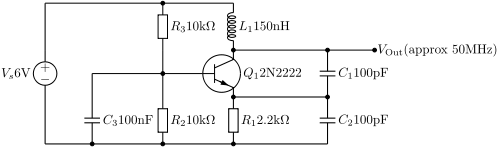
\includegraphics[width=0.5\textwidth]{images/colpitts.png}

\tiny{\url{http://en.wikipedia.org/wiki/File:NPN_Colpitts_oscillator_collector_coil.svg}}
\end{centering}
\begin{itemize}
\item Colpitts gets the feedback via a capacitive divider

\item VFO usually based on Colpitts due to stability
\end{itemize}
\end{frame}

\begin{frame}{Hartley}{}
\begin{centering}
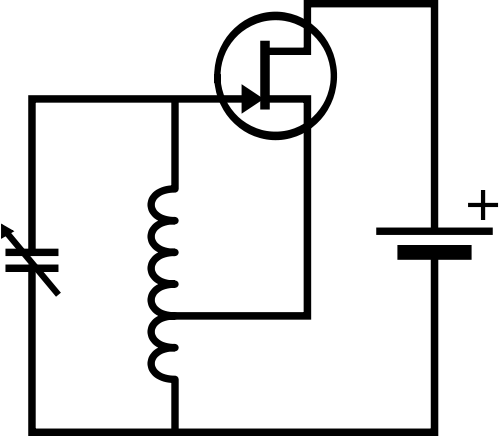
\includegraphics[width=0.5\textwidth]{images/hartley.png}

\tiny{\url{http://en.wikipedia.org/wiki/File:Hartley_osc.svg}}
\end{centering}
\begin{itemize}
\item Hartley gets the feedback via a tapped coil
\end{itemize}
\end{frame}

\begin{frame}{Pierce}{}
\begin{centering}
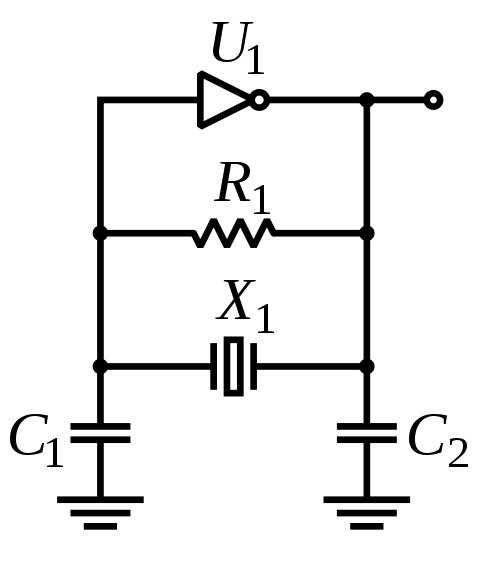
\includegraphics[width=0.5\textwidth]{images/pierce.png}

\tiny{\url{http://en.wikipedia.org/wiki/File:Pierce_oscillator.svg}}
\end{centering}
\begin{itemize}
\item Pierce gets the feedback via a capacitive coupling
\item Pierce is usually used for crystals
\end{itemize}
\end{frame}

\begin{frame}{Phase locked loop (PLL)}{}
\begin{itemize}
\item Controller that generates an output signal with phase related to phase of an input signal.
\item Analog and digital implementations.
\item Analog form is a phase detector and a VCO.
\end{itemize}
\end{frame}

\subsection{RF Power Amp}
\begin{frame}{Grounded Grid amplifier}{}
\small{Repeated from last time}
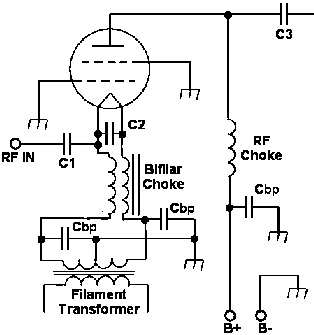
\includegraphics[width=0.5\textwidth]{images/gg1.jpg}
Image taken from \url{http://wb0nni.dakotamade.com/ggbasic.html}.  See there for discussion, also the answer to the grounded grid questions
\end{frame}

%\begin{frame}{RF amps}{}
%include graphic simple CW transmitter

%Inductive coupling may be used between oscillator and RF power amp.  This forms another tuned circuit to further reduce undesired frequencies (harmonics)

%Note uses of RF chokes to keep RF out of the power supply

%Neutralization may be required on some vacuum tube amps to prevent parasitic oscillation due to capacitances inside the tube.  Couple a small amount of the output back to the input 180 degrees out of phase (negative feedback)

%Neutralization is indicated by minimum change of grid current while output circuit is tuned.

%\end{frame}
\subsection{Modulation}
\begin{frame}{Modulation types}{AM/SSB}
\begin{itemize}
\item Amplitude Modulation (AM)
\begin{itemize}
\item output is carrier and two sidebands, but really, all the info is in one sideband
\end{itemize}
\item Balanced modulator
\begin{itemize}
\item removes the carrier
\end{itemize}
\item Single Side Band (SSB)
\begin{itemize}
\item effective 6db gain in the transmitter and 3dB in the receiver.
\end{itemize}
\end{itemize}
\end{frame}

\begin{frame}{Modulation types}{FM}
\begin{itemize}
\item Frequency Modulation (FM)
\begin{itemize}
\item Frequency varies linearly with voltage
\item Modulation Index: $x=\frac{D}{f_m}$, 
\item Deviation Ratio: $dr=\frac{D}{f_{max}}$.
\item Necessary Bandwidth: $B=2M+2D$
\end{itemize}
\end{itemize}
\end{frame}

\begin{frame}{Modulation types}{FM}
\begin{itemize}
\item Phase Modulation
\begin{itemize}
\item Phase varies linearly with voltage
\item Of necessity, this also varies frequency, but not linearly with voltage
\item PM emphasises higher frequencies
\item Commercial standards based on PM
\item Preemphasis in the {\em FM transmitter} artifically boosts high frequencies
\item Deemphasis in the {\em FM receiver} restores the original signal 
\end{itemize}
\end{itemize}

\end{frame}

\begin{frame}{Modulation types}{}
Intermodulation interference

\begin{itemize}
\item Occurs when nonlinear mixing takes place between two transmitted frequencies.  Usually in the final amp.
\item Most common frequencies are 2A-B, and 2B-A
\end{itemize}
\end{frame}

\begin{frame}
Spread spectrum:  see notes
\end{frame}

\subsection{Repeater}
\begin{frame}{Repeater}{}
Notes taken from the Exhaminer comments

"The Carrier Operated Relay (COR) is the circuit which detects an incoming signal at the receiver.  In a simplistic repeater, the COR would in turn activate the transmitter.  In real-life, the COR signal is taken through a controller where a time-out timer (to prevent overly long transmissions), a "tail" timer (hang time, to keep the repeater on the air between exchanges), a courtesy tone (or "tail beep", to signal the reset of the time-out timer) and an identifier (to transmit the repeater's call sign) are implemented."

"In the context of a repeater installation, a duplexer is a specialized filter which allows operating the receiver and transmitter simultaneously on the same antenna.  The duplexer is built with four or more quarter-wavelength cavity resonators.  The duplexer provides isolation ( 90 dB or more on 2m ) between the receive and transmit paths at the expense of insertion loss."

Intermodulation is usually cited in the context of a repeater.
\end{frame}

\section{Codes}
\begin{frame}{Codes}{AMTOR}
\begin{itemize}
\item AMTOR - Amateur Teleprinting Over Radio
\item MODE A - ARQ - (automatic repeat request) retransmission of the group of characters will occur automatically if the transmission is not acknowledged.
\item MODE B - FEC - (Forward error correction) redundancy, hamstudy says each character is sent twice.
\item Generally replaced by PSK31, etc now.
\end{itemize}
\end{frame}
\begin{frame}{Codes}{ASCII}
ASCII - American Standard Code for Information Interchange - 8 bit transmission (in the questions), but 7-bit by orig. definition
\begin{centering}
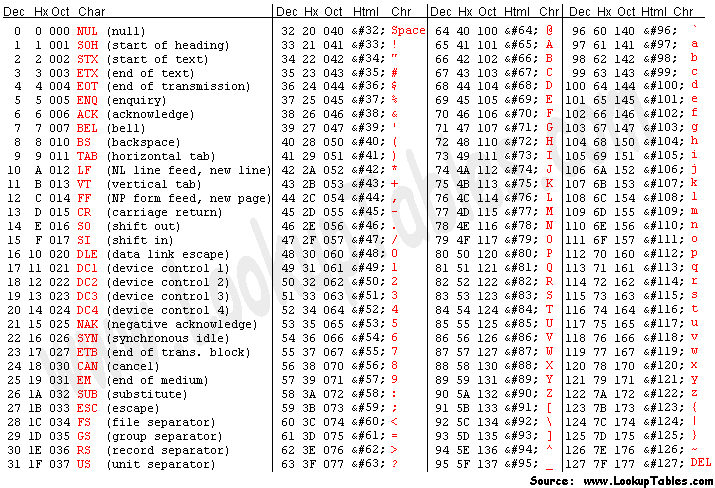
\includegraphics[width=0.6\textwidth]{images/asciifull.png}

\tiny{\url{www.asciitable.com}}
\end{centering}
\end{frame}

\begin{frame}{Codes}{AX.25}
\begin{itemize}
\item AX.25 - packet radio protocol.
\item Occupies first, second and third layers of OSI networking model (physical, data and network)
\end{itemize}
\end{frame}

\begin{frame}{Codes}{BAUDOT}
BAUDOT - 5 bit transmission - One case for text, shift between figure and text mode.
\begin{centering}
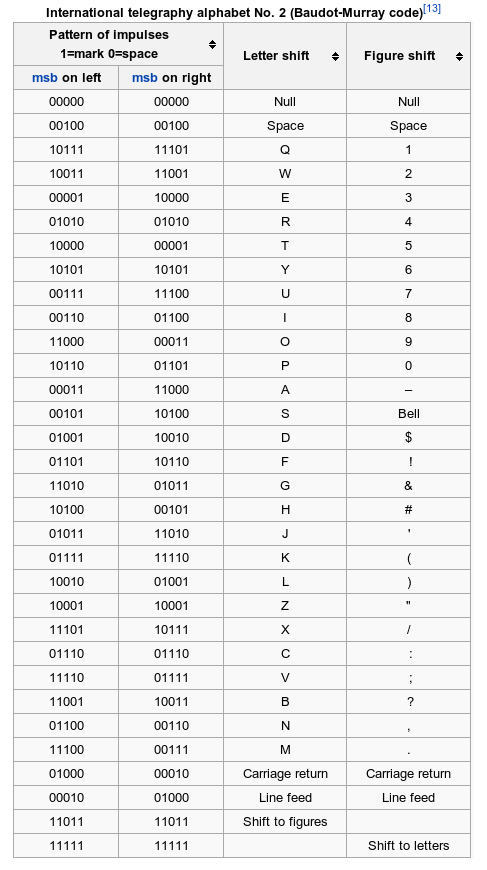
\includegraphics[width=0.3\textwidth]{images/baudot_ita.png}

\tiny{\url{http://en.wikipedia.org/wiki/Baudot_code}}
\end{centering}
\end{frame}

\begin{frame}{Codes}{Morse}

CW - Morse code.  Note variable length per character - more frequently used characters are shorter.
\begin{centering}
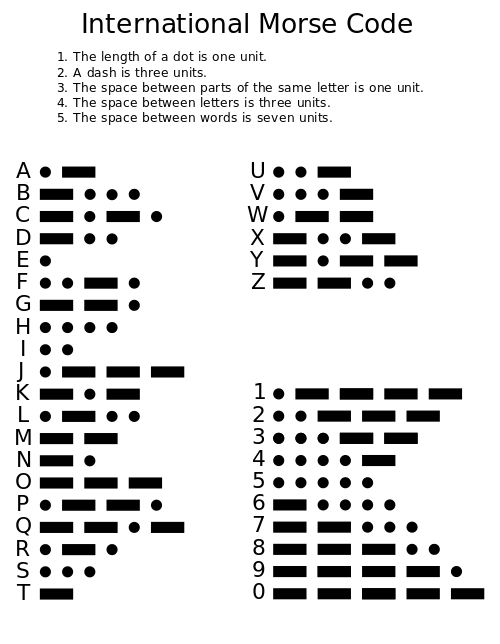
\includegraphics[width=0.4\textwidth]{images/morse.png}

\small{\url{http://en.wikipedia.org/wiki/File:International_Morse_Code.svg}}
\end{centering}
\end{frame}


\section{Signal Processing}
\begin{frame}{Signal Processing}
(See the HamStudy notes)
\end{frame}


%%%%%%%%%%%%%%%%%%%%%%%%%%%%%%%%%%%%%%%%%%%%%%%%%%%%%%%%%%%%%%%%%%%%%%%%%%%%%%%%%%

%\section{Modulation}

%\subsection{Rectifiers}
%\begin{frame}{Rectifiers}{}
%\end{frame}

%%%%%%%%%%%%%%%%%%%%%%%%%%%%%%%%%%%%%%%%%%%%%%%%%%%%%%%%%%%%%%%%%%%%%%%%%%%%%%%%%%
\end{document}
 
